\documentclass[a4paper, 11pt]{article}
\usepackage{comment}
\usepackage{fullpage}
\usepackage[german]{babel}
\usepackage{graphicx}

\begin{document}
\noindent
\large\textbf{Programmierübung 2} \\
\textbf{Bloom Filter} \\
\normalsize FHNW Brugg Windisch - Modul Diskrete Stochastik \\
Bearbeitet von Anessollah Ima und Jonathan Bättig\hfill Datum: 25.11.2019 \\
 

\section*{A) Idee des Bloom Filters}
Der Bloom Filter ermöglicht es sehr sehr schnell zu prüfen, ob ein Elemen in einer Liste vorhanden ist oder nicht. Wenn der Bloom Filter behauptet, dass ein Element noch nicht vorhanden ist, so stimmt diese Aussage immer zu 100\%. Wenn die Berechnungen des Filters allerdings ergibt, dass das Element bereits vorhanden ist, so darf man dem Filter nicht trauen. Es ist möglich, dass ein Element trotzdem noch nicht vorhanden ist. Der Bloom Filter ist also eine probabilistische Datenstruktur.
\cite{Wikipedia}
\cite{Youtube}

\subsection{Vorteile}
\begin{description}
\item[-]
Der Bloom Filter benötigt sehr wenig Speicherplatz.
\item[-]
Die Implementation des Bloom Filters ist simpel.
\item[-]
Die asymptotische Komplexität beträgt nur O(k), wobei k die Anzahl Hash Funktionen ist.
\end{description}

\subsection{Nachteile}
\begin{description}
\item[-]
Das Resultat des Bloom Filters ist nicht immer eindeutig.
\item[-]
Der Bloom Filter speichert keine Daten.
\end{description}

\section*{B) Konkretes Praxisbeispiel}
Im Bitcoin Netzwerk verwenden einige Clients den Bloom Filter um Transaktionen innerhalb des Netzwerks zu prüfen. Bei der Überprüfung muss dank des Bloom Filters keine komplette Kopie des Blockchain aufbewahrt werden.
\cite{Medium}

\section*{C) Vorgehensweise bei der Berechung der Fehlerwahrscheinlichkeit}

\cite{Testsite}
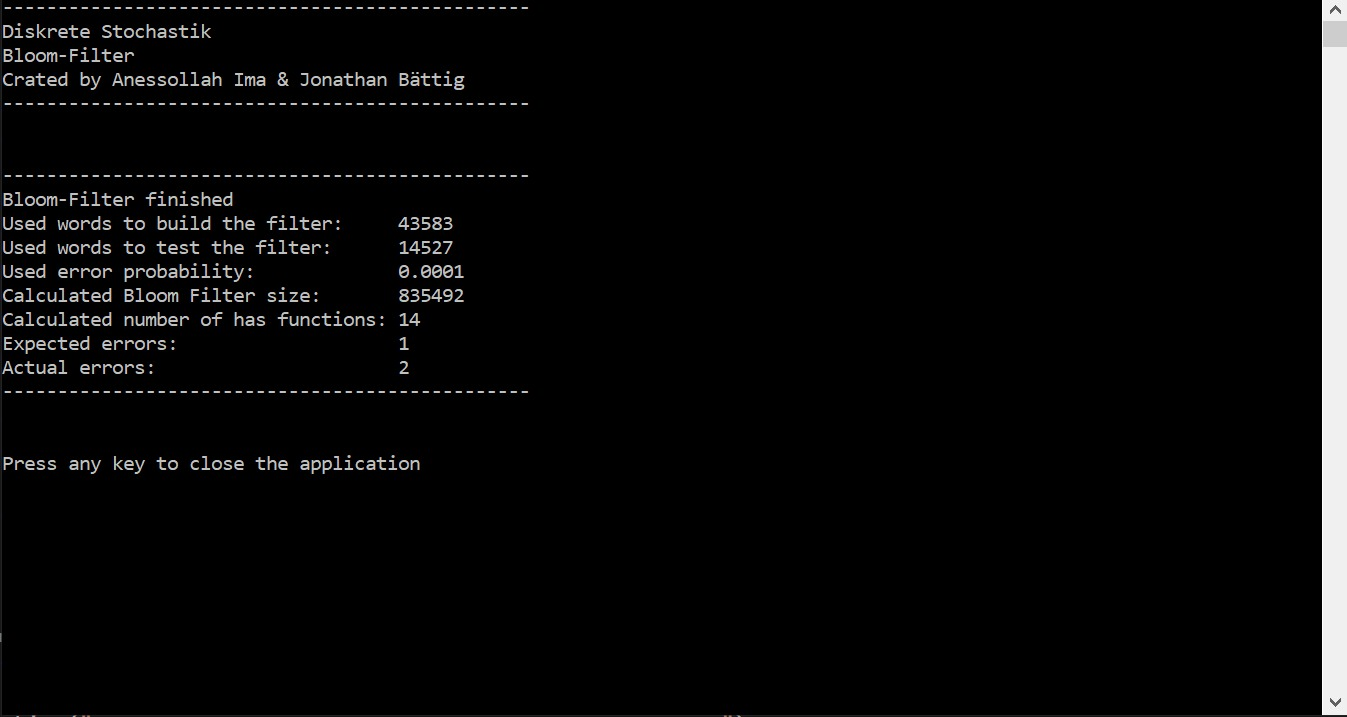
\includegraphics[width=\textwidth]{Program.jpg}

\begin{thebibliography}{9}
\bibitem{Wikipedia} (https://en.wikipedia.org/wiki/Bloom\_filter)
\bibitem{Youtube} (https://www.youtube.com/watch?v=Bay3X9PAX5k)
\bibitem{Medium} (https://medium.com/@tara.annison/bloom-filters-and-spv-nodes-within-the-bitcoin-blockchain-66c36ea673f2)
\bibitem{Testsite} (https://hur.st/bloomfilter/)
\end{thebibliography}

\end{document}